\chapter{Rendering}
\label{chapter:rendering}
This chapter will describe how the IRCs from the previous chapter can be used to improve path tracing.
We will use the terms "'BSDF sampling"' and "IRC sampling"' for the process of sampling an incident direction and its probability from a surface point's BSDF or corresponding IRC respectively. How samples can be generated from a BSDF will not be discussed here any further.\newline
The first part of this chapter will cover generating samples and probabilities from an IRC. The second part combines IRC sampling with BSDF sampling or NEE using Multiple Importance Sampling. In the end we evaluate the results.


\section{Sampling Caches}
\subsection{Path Extension}
\label{path extension}
As described in chapter \ref{chaper:PathTracing}, path tracing creates random paths starting at the camera and traces these paths across the scene until either a light source is hit or the path leaves the geometry. To do that, we need to choose a new direction every time the path hits a surface at an intersection point $x$. This is normally done by sampling an outgoing direction from the surface's BSDF. In that case the applied pdf is proportional to the BSDF term from the rendering equation. The goal of our IRCs is to use a pdf which approximates the incident radiance $L_i(\omega_i,x)$ instead of the BSDF.

Our basic algorithm for sampling a new outgoing direction proportional to the irradiance consists of several steps: Picking an appropriate cache, sampling a direction and computing its probability.\\
So, first we have to choose the cache we want to use. Sometimes, especially at corners, thin walls or curved surfaces, the closest cache can have another normal than the surface at $x$ itself. If the deviation is small enough, the cache can be used anyway. However, if the cache's rotation is too severe, it might be better to pick one of the next closest caches more parallel to the surface at $x$. We chose $0.9$ to be the threshold for the cosine between the cache's and surface's normal and never considered more than the 5 closest caches.\newline
This may seem arbitrary, but in our example scenes most caches violating that threshold had a cosine of $0$ or less to the surface. Plus whenever a cosine was positive but below 0.9, some of the other closest caches often exhibited bigger values. We also didn't experience any problems with spheres, since the caches were always placed densely enough.

With more complex scenes and small spheres in rarely lit areas that are not seen by the camera directly but hit many times for indirect lighting, one would have to test if 0.9 is still a good choice or if a smaller values would be a better option. On the other hand, if only few photons arrive in a region in the first place, it might prove more useful to just use normal BSDF sampling there.

Instead of always choosing the closest cache (or that one of the 5 closest ones with the best cosine), we decided to randomly pick one of those caches that was among the 5 closest to $x$ and also had the best cosine value. In most cases these were all 5 closest caches with a cosine of 1. This process is depicted in algorithm \ref{algopickcache}.\newline

\begin{algorithm}
\caption{Pick Cache}\label{pickCache}
\begin{algorithmic}[1]
\Procedure{pickCache}{$surfacePoint$}
\State $cacheList \gets kdTreeCaches.getKClosestCaches(5,surfacePoint.position)$
\State $bestCos \gets -1$
\For {$i=0$ to $4$}
\State $currentCache \gets cacheList\lbrack i\rbrack$
\State $currentCos \gets cos(currentCache.normal, surfacePoint.normal)$
\If{$currentCos > bestCos$} 
\State $bestCos\gets currentCos$
\State $bestCache \gets currentCache$
\ElsIf {$currentCos == bestCos$ $\wedge$ $getRandomNumber() > 0.6$}
\State $bestCache\gets currentCache$
\Else
\EndIf
\EndFor
\If {$bestCos > 0.9$}
\State \textbf{return} $bestCache$
\EndIf
\State \textbf{return} $null$ \Comment {sample BSDF instead}
\EndProcedure
\end{algorithmic}
\label{algopickcache}
\end{algorithm}


Line $7$ ensures that we only use caches with the highest cosine value. Line $10$ takes care that we pick one of the best caches at randon, with closer caches having a higher probability of being chosen. If all five closest caches are rotated too much towards the surface at $x$, we resort to BSDF sampling just this once.

As it turns out, choosing between the 5 closest caches instead of just using the closest cache (if its cosine is high enough) consumes a third of the total computation time \ref{durations}. Plus we could not see any difference in the resulting images as long as enough IRCs were available. Maybe picking one of 5 caches is more useful for more complex scenes than our simple examples, where there is more curved geometry or edges.

After a cache is chosen, the next step is sampling a direction from that cache. For that purpose three random numbers between 0 and 1 are required. The first one is used to pick a texel from the cache's environment map. To do that we look for the field in the cache's $cdf\_map$ (see chapter \ref{storing cache}) with a value bigger or equal to the random number. The other two are needed to sample a point within the texel. This point is converted to a direction (reverse equations \ref{planar_projection} and \ref{planar_projection2}).

As we always need the probability of the sampled direction whenever a direction is sampled, algorithm \ref{sampleCache} also returns the probability for sampling the direction. Note that while the cdf was created from a pdf that sums up to one, the returned probability is measured over solid angle and was computed after the cdf was created.\newpage


\begin{algorithm}
\caption{Sample Direction from Cache}\label{sampleCache}
\begin{algorithmic}[1]
\Procedure{sampleDirection}{$cache,pdfValue,rand1,rand2,rand3$}
\State $texel\_index \gets $ \Call{binarySearch}{$cache.cdf,rand1$}
\State $pdfValue \gets cache.pdf\_map\lbrack texel\_index\rbrack$
\State $texel.x \gets texel\_index \% cache.mapWidth + rand2$
\State $texel.y \gets texel\_index / cache.mapWidth + rand3$
\State $Vector3D$ $direction \gets cache.texelToDirection(texel)$
\State $direction \gets cache.coordinateSystem.toWorld(direction)$
\State \textbf{return} $direction$
\EndProcedure
\end{algorithmic}
\end{algorithm}


We use binary search to find the index of the sampled texel in our $cdf\_map$ more efficiently. This index yields the probability for its texel from the $pdf\_map$, we write that probability to $pdfValue$ so it can be used later on. \\
Note that the pdf is designed for texels with an area of $1\times 1$, so we can get a random point within that texel from lines $4$ and $5$. Line $6$ converts this point to a point in $\lbrack -2,2\rbrack \times \lbrack -1,1\rbrack$ (or $\lbrack -2,0 \rbrack \times \lbrack -1,1\rbrack$, see chapter \ref{envmap param}) and then to a direction in local coordinates (the upper axis matches the top of the octahedron), which is converted to a direction in global coordinates in line $7$.


After a (global) direction $\omega$ is sampled, we can continue the path along $\omega$. The last thing left to do is to weight the energy carried along the path. Therefor we have to evaluate the BSDF at $x$ with $\omega$ as incoming (!) direction $\omega_i$ and appoint the direction where the path came from as outgoing direction $\omega_o$. The energy carried along the path can be weighted just as in algorithm \ref{assembleenergy} according to equation \ref{geoweg} as follows:\\

\begin{algorithm}
\caption{Weight path energy for Monte Carlo integration}
\label{weight1}
\begin{algorithmic}
\State $bsdfValue \gets x.bsdf.eval(\omega_i,x,\omega_o)$
\State $cos \gets cos(\omega_i,x.normal)$
\State $pathEnergy \gets pathEnergy \cdot bsdfValue \cdot cos / pdfValue$
\end{algorithmic}
\end{algorithm}

Note that the BSDF technically evaluates directions represented in local coordinates at $x$, so we would actually have to convert the directions from world to local coordinates first. Fortunately, if the cosine of the used cache happens to be $1$, we can skip the transformation of $\omega_i$ and just use the local cache coordinates from line 6 in algorithm \ref{algopickcache} instead, as long as the rendering framework can guarantee consistency of both coordinate systems.

However, there are cases when IRC sampling is not a good option: At specular surfaces, only light from one direction (or two for transmitting materials) actually contributes to the integral to compute. It is therefore unnecessary to randomly sample several directions, we can directly sample the one (or 2) important direction from the surface's BSDF. Note that in chapter \ref{placing caches} we only placed caches at non-specular surfaces: The cache positions were created either from photons (which are only stored for non-delta BSDFs) or from camera rays (which were traced across the scene until a surface with a non-delta BSDF was found).\newline
It might also happen that there are no caches nearby, or that the closest caches are rotated too much to provide useful information. In these cases we fall back on conventional BSDF sampling. 




\newpage
\subsection{Computing probabilities for given directions}
\label{computePdf}
For simple path tracing with implicit paths from IRC sampling only, the previous section contains all the steps we need. However, if we want to combine IRC sampling with NEE or BSDF sampling, we also need to be able to extract a probability value from a cache for a given direction in order to compute MIS weights.\newline
Therefor we first pick a cache just like in algorithm \ref{pickCache}. Next we convert the direction to local coordinates in the cache's coordinate system and then on to texture coordinates according to equations \ref{planar_projection} and \ref{planar_projection2}. A simple access to the cache's $pdf\_map$ at the computed texel yields the probability for having sampled the given direction with this cache, measured over solid angle.









\newpage
\section{Combining BSDFs and Caches}
\label{combining BSDFs and caches}
The figures in chapter \ref{importance_sampling_options} showed the flaws of choosing only one local sampling method. Figure \ref{veach_mis} already compared BSDF sampling and NEE. And while our IRCs are capable of rendering caustics, they also produce a considerable amount of noise. This noise can be worse or better than the noise we get from sampling the BSDF, depending on the scene and the quality of the caches.\\
As opposed to combining BSDF sampling and NEE, BSDF and IRC sampling cannot be done at the same time: Since we use path tracing, we don't want to split up a path into two paths whenever we hit a surface. Hence we need a way to choose between BSDF and IRC sampling and a way to combine them.

We use the BSDF's roughness to decide whether to sample the BSDF or IRCs. If the BSDF is ideally diffuse, the BSDF itself will have the same value for every direction and we cannot gain much information or increase the integrand by sampling the BSDF. On the other hand, if we hit a (near) delta BSDF, for most of the directions the incident radiance will have (almost) no contribution due to the BSDF being close to zero for most angles.

There are certain reasons not to importance sample for irradiance at all. One are delta-BSDFs: Whenever a surface is perfect specular, perfect transmitting or both, there is only one (or two) directions that actually contribute light to the current path. Whenever we hit a surface with a delta-BSDF, we will automatically only sample the BSDF with MIS weight 1, and also skip the next event estimation (if included) completely, since the probability of it having any contribution at all is zero.

Another case depends on the placement of the caches. Sometimes there might just be no caches available close to the current surface point. In simple scenes, this is almost never the case, but we can never be sure to prevent this completely, especially with more complex scene geometry.\newline
A similar case is a more complex, curved geometry. For example, consider placing caches on a sphere. Since we can never cover the whole surface area of a sphere with points, there will always be points that are hit by camera rays but have no cache at their exact position. There might be a cache very close to them, but judging from an analytical point of view the angle between their normals will never be 0. If that angle is still small (or the cosine between them big) enough, we can ignore the deviation and still use the cache, for everything we have was only approximated in the first place. We allowed a small margin of difference between the cache's normal and the surface point's normal (see \ref{path extension}). But whenever the cosine is smaller than 0.9 we ignore the caches and sample the BSDF with weight 1.\newline
If the cosine of the selected cache is bigger than 0.9 but less than 1, the outgoing direction of our path can be sampled from the IRC. It will however be converted to global and then to local coordinates at the intersection point in order to evaluate the BSDF at that point. Note that the sampled drection was represented in local cache coordinates at first and would also have been converted to global coordinates for a cosine of 1 anyway. See algorithm \ref{pickCache} on how caches are picked depending on their cosine to the surface normal at the current intersection point.




\subsection{Multiple Importance Sampling of BSDFs and IRCs}
\label{mis_BSDF_irc}
As implied in the previous segment, we will only actually combine BSDF and IRC sampling whenever we hit a surface with a non-delta BSDF and if a cache with a good enough cosine to the surface normal is near. In all other cases we continue our path by generating a sample from the BSDF with MIS weight 1.\newline
In this section we show how we decided on a probability to select either BSDF or IRC sampling, and how to compute the MIS weights for each of them.

The Mitsuba Renderer, which was used as a framework to implement this work, offers the roughness of a BSDF in the form of a floating point value $\in\lbrack 0,1\rbrack$. A roughness value of $\infty$ is used in addition to indicate perfectly diffuse surfaces.\newline
We decided that even if a surface is completely diffuse, BSDF sampling should not be ignored completely. Then again we never want to pick IRC sampling at perfectly specular surfaces for reasons explained above. So we decided on $\alpha = min($roughness$,0.9)$ as a threshold for randomly selecting BSDF or IRC sampling.

Chapter \ref{multiple importance sampling} explained how $n$ exclusive sampling techniques can be combined with the one-sample model. In our case BSDF sampling is chosen with probability $1 - \alpha$ and IRC sampling with probability $\alpha$. These probabilities obviously sum to one, they match $c_1$ and $c_2$ in equation \ref{onesample}.\newline
Assume we generated a random number $>\alpha$ and sampled some direction $\omega$ with a probability $p_{bsdf}$ from the BSDF. To compute that sample's MIS weight we also need to compute the probability $p_{cache}$ for having sampled $\omega$ from the chosen cache (see chapter \ref{computePdf}). With both pdfs being measured over solid angle, the weighting function $w_{bsdf}$ for the sampled direction can now be determined by the balance heuristic:

\begin{equation*}
w_{bsdf} = \frac{p_{bsdf}}{p_{bsdf}+p_{cache}}.
\end{equation*}

According to equations \ref{onesample} and \ref{geoweg} the total weight we have to multiply to the energy carried along the path is

\begin{equation*}
pathEnergy ^*= \frac{w_{bsdf}}{(1-\alpha)} \cdot \frac{f_s \cdot cos(\omega)}{p_{bsdf}}.
\end{equation*}

Assuming that the path's energy was already weighted similar to algorithm \ref{weight1} with $p_{bsdf}$ as $pdfValue$ before, we can weight the path energy like this: \newline

\begin{algorithmic}
\State $totalWeight \gets \frac{p_{bsdf}}{(1-\alpha) \cdot (p_{bsdf}+p_{cache})}$
\State $pathEnergy \gets pathEnergy \cdot totalWeight$
\end{algorithmic}


If the initial random number was $\leq \alpha$ and \ref{weight1} was already executed, the MIS weight for IRC sampling can be computed accordingly:\newline %TODO accordingly ist blöd...

\begin{algorithmic}
\State $totalWeight \gets \frac{p_{cache}}{\alpha \cdot (p_{bsdf}+p_{cache})}$
\State $pathEnergy \gets pathEnergy \cdot totalWeight$
\end{algorithmic}

\section{Combining NEE and Caches}

We also combined NEE with IRCs. Basically we replaced BSDF sampling with generating samples from the IRCs, and used the probabilities from the caches instead of the probabilities from the BSDF.\\
At ideal specular surfaces (those with a delta BSDF) we still used BSDF sampling instead of the IRCs. The probabilities won't matter in that case, as the MIS weights at delta-BSDFs are $1$ for BSDF sampling and $0$ for any other strategy anyway. Theoretically we also rely on BSDF sampling if no caches are close enough or the closest caches are rotated too much, but this was never the case with our test scenes.












\section{Evaluation}
All scenes are original or modified versions of the scenes available on the Mitsuba renderer's download website \cite{mitsuba}. All caches had a resolution of $16\times 16$ per hemisphere, they were filtered bilinear while they were filled and filtered with a Gaussian filter afterwards.

We used the following scenes:


\begin{itemize}
\item \textbf{Glass Spheres}

With this scene, BSDF sampling combined with NEE (figure \ref{kugel_BSDF}, left) produced the worst result, i.e. the image with most noise around the caustics. The best image resulted from combining NEE and IRCs - the IRCs perform better than BSDF sampling around the caustics, and NEE produces close to zero noise in the remaining areas (even with less samples per pixel).\\
Figures \ref{kugel_nee_caches} and \ref{kugel_BSDF} each had 200k photon paths, 20k caches, 2k photons per cache and 256 samples per pixel.

\item \textbf{Mirror Boxes}

The images with the mirror boxes were rendered with 150k photon paths, 20k caches, 1k photons per cache and 128 samples per pixel. Note that with the glass spheres, the image rendered with NEE and IRCs showed less noise than the other two images. Here, the overall noise is roughly the same for figure \ref{spiegel_nee_caches} (NEE and IRCs) and the left part of figure \ref{spiegel_BSDF} (NEE and BSDF). The caustics are still the smoothest with NEE and IRC sampling.

\item \textbf{MIS Test Scene}

This scene was initially used by Veach to illustrate the effects of Multiple Importance Sampling, see figure \ref{veach_mis}. The combination of NEE and BSDF sampling is the best choice for this scene; in figure \ref{veach_mis} there is almost no noise even though it was rendered with only 64 samples per pixel. It seems like combining BSDF sampling and NEE covers the cases of direct lighting pretty well and there was never much room for improvement in the first place.\\
As it turns out, either combination of IRCs with BSDF sampling or NEE results in worse images. A possible reason for this is that our caches have a resolution of only $16 \times 16$ texel for one hemisphere and are too inaccurate for the smallest light source, so they don't perform well on the left. Plus, we don't expect them to work fine for the upper board either, for reasons explained in section \ref{combining BSDFs and caches}.\newline
The images were rendered with 150k photon paths, 20k caches, 1k photons per cache and 64 samples per pixel. \ref{veach_mis} contains the image for BSDF sampling and NEE, but figure \ref{veach_ircs} should suffice to see the reasons why both combinations with IRCs are inferior.\\
Maybe combining NEE, BSDF sampling and IRC sampling results in a more robust algorithm that can handle scenes like this one as well.

\item \textbf{Glass Egg on Table}

Veach used this scene in \cite[chapter 10]{veachdiss} to demonstrate the benefits of bidirectional path tracing over standard path tracing as we used it. While bidirectional path tracing is without a doubt the better choice for this scene, the combination of NEE and IRC sampling results in a distinctly smoother image than the conventional combination of NEE and BSDF sampling (shown in figure \ref{bidir_ircs}).
\end{itemize}

\newpage
\subsection{Comparison of Different Sampling Strategies}



 \begin{figure}[h!]
 \centering
 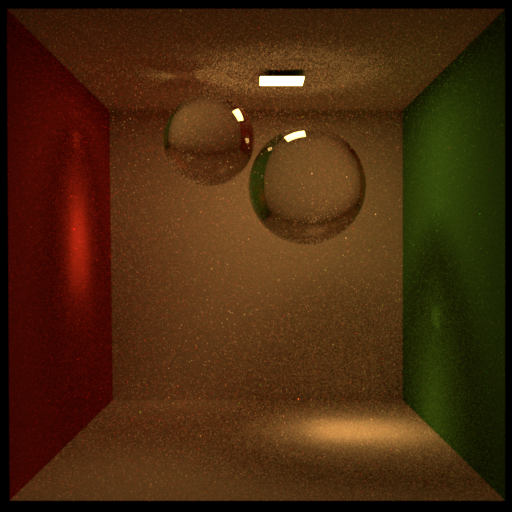
\includegraphics[width=0.5\textwidth]{bilder/kugelbox/nee&caches_200k20k2k_256spp.png}
\caption{NEE and IRC sampling: The IRCs handle the caustics, and NEE takes care of an overall smooth appearance.}
 \label{kugel_nee_caches}\end{figure}


 \begin{figure}[h!]
 \centering
 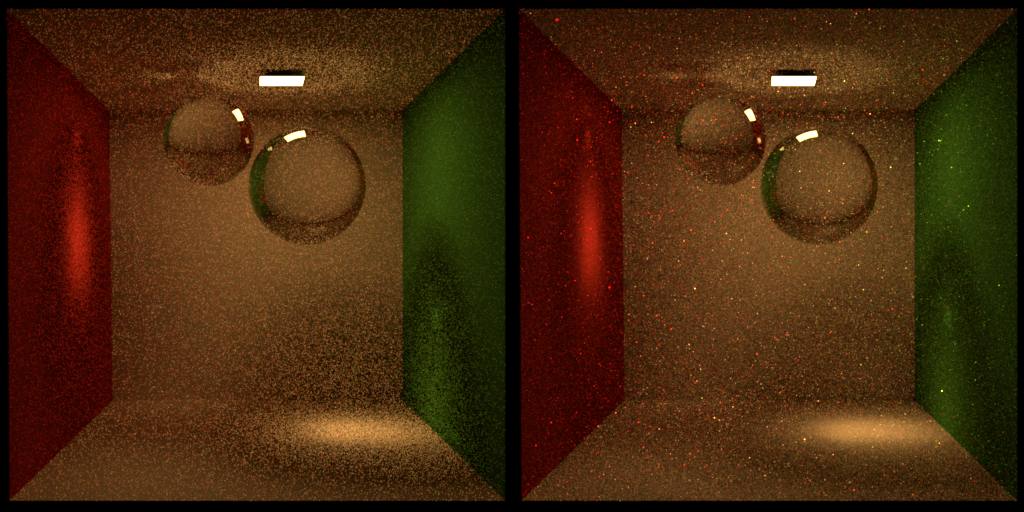
\includegraphics[width=1\textwidth]{bilder/kugelbox/bsdfcombos.png}
\caption{Left: NEE and BSDF sampling. In comparison to IRCs, BSDF sampling produces more noise in the caustics. The general noise produced by BSDF sampling consists of darker dots, while the noise of IRCs are colored sparks which can be cancelled out easier by NEE.\newline
Right: BSDF sampling and IRCs. The caustics look better than on the left, but the overall noise is worse.}
  \label{kugel_BSDF}\end{figure}

 \begin{figure}[h!]
 \centering
 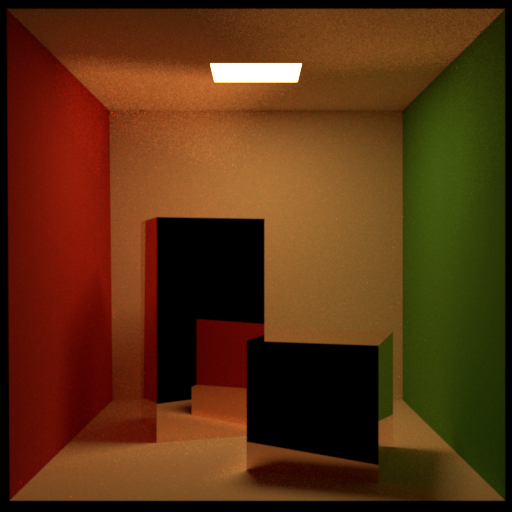
\includegraphics[width=0.5\textwidth]{bilder/spiegelbox/nee&caches_150k20k1k_128spp.png}
\caption{NEE and IRC sampling.}
  \label{spiegel_nee_caches}\end{figure}

 \begin{figure}[h!]
 \centering
 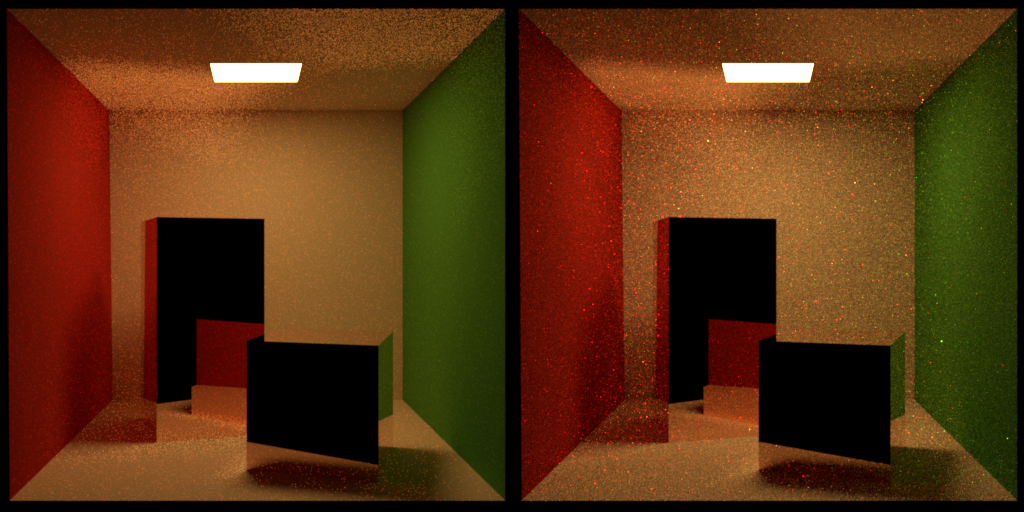
\includegraphics[width=1\textwidth]{bilder/spiegelbox/bsdfcombos_128spp.png}
\caption{Left: NEE and BSDF sampling. Just as with the glass spheres, the caustics show more noise than figure \ref{spiegel_nee_caches}. The noise on the walls is roughly the same, which might be the result of the brighter light source.\newline
Right: BSDF sampling and IRCs. While the caustics are smooth, there is notable noise from the IRCs.}
  \label{spiegel_BSDF}\end{figure}


 \begin{figure}[h!]
 \centering
 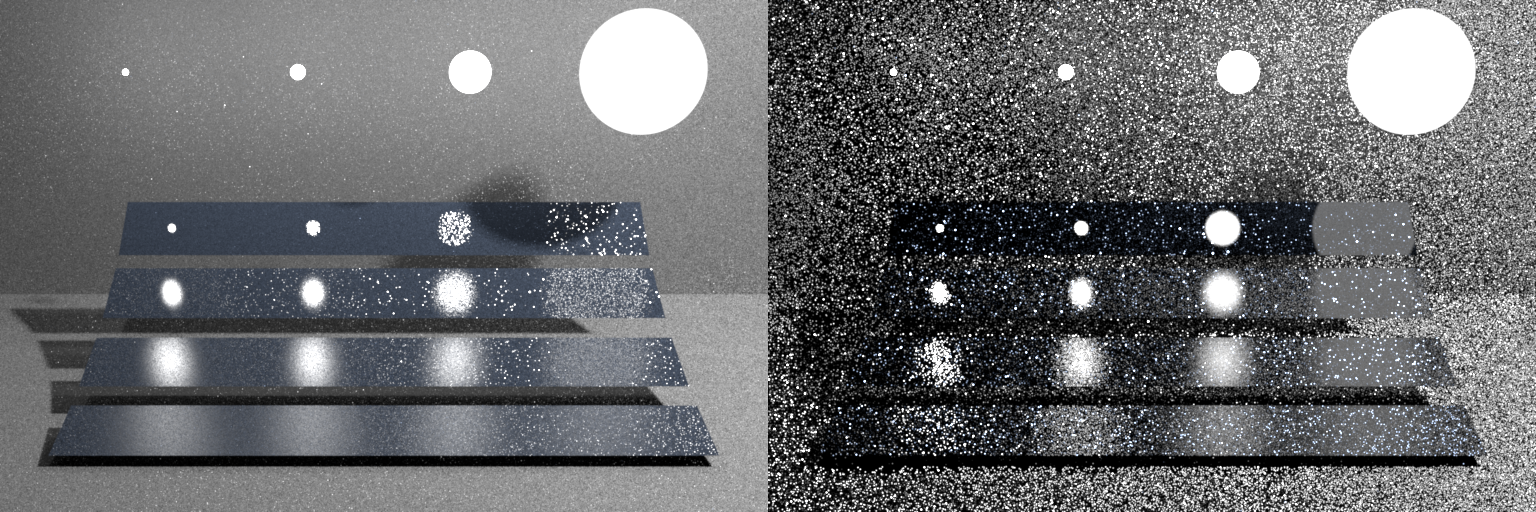
\includegraphics[width=1\textwidth]{bilder/veach/cachecombos_64spp.png}
\caption{Left: NEE and IRCs. Right: BSDF sampling and IRCs.}
  \label{veach_ircs}\end{figure}

 \begin{figure}[h!]
 \centering
 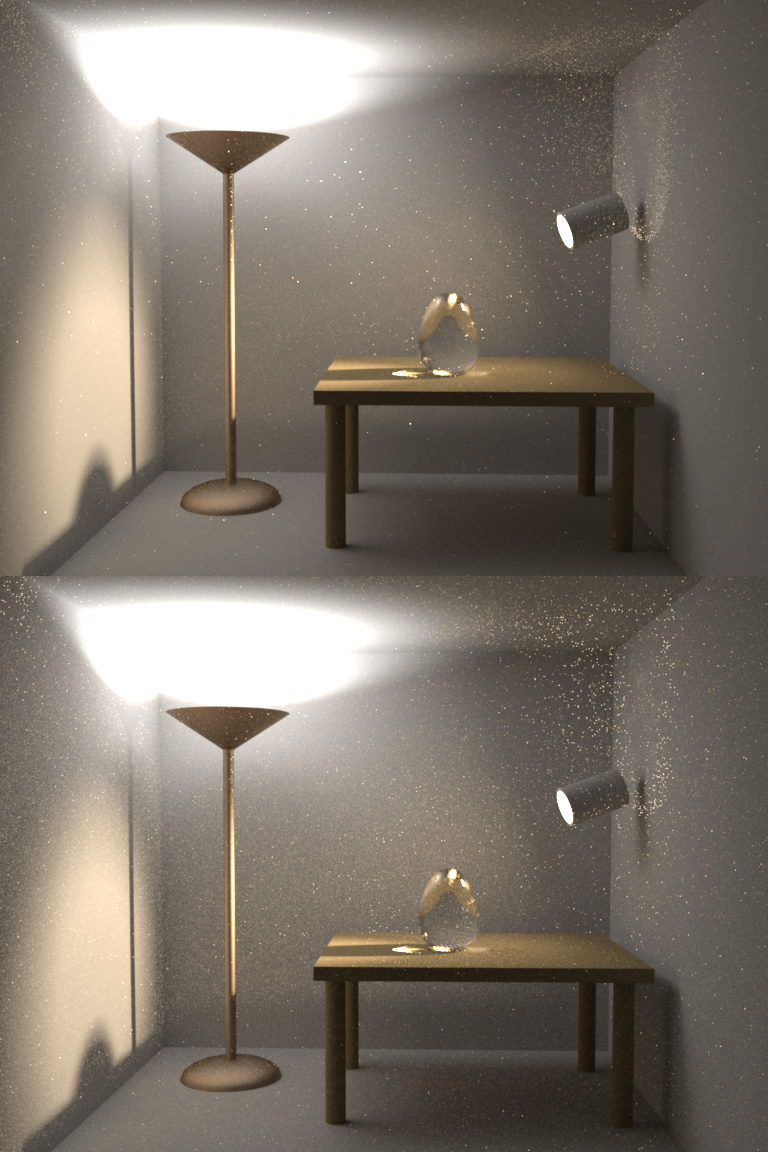
\includegraphics[width=0.7\textwidth]{bilder/bidir/vergleich.png}
\caption{Top: Rendered with NEE and IRCs, 250k photon paths ($\approx$ 1.500.000 photons), 30k caches, 2k photons per cache, 4096 samples per pixel.\newline
Bottom: Rendered with NEE and BSDF sampling, 4096 samples per pixel.}
  \label{bidir_ircs}\end{figure}



\clearpage



\subsection{Different Cache Configurations}\label{dcc}
In this section we investigate the impact of a different amount of photon paths, caches and photons per cache.\\
We found that environment map resolutions of $4\times 4$ and $8\times 8$ were too small, while a resolution $16\times 16$ produced decent results that $32\times 32$ was not able to improve.\\
As a limitation, we always created the same amount of camera caches (one for every $8\times 8$ pixel block). All additional caches were created from photons. The images below are rendered with NEE and IRC sampling, as this produced the best results.\\
The preprocessing time is proportional to the number of caches and number of photons per cache. The photon tracing pass itself is several orders of magnitude faster than filling the caches.


As it turns out, for simple scenes where most of the geometry is visible anyway the camera caches are mostly sufficient. However, there may appear artefacts along the edges. These can be removed by either picking one of the five closest caches with a better angle (see algorithm \ref{algopickcache}), or by adding more caches. For example, the glass sphere scene with camera caches only had 3768 caches and noticable artefacts along the edges within the caustic. These were gone when the same scene was rendered with 20k caches (figure \ref{artefacts}).



 \begin{figure}[h!]
 \centering
 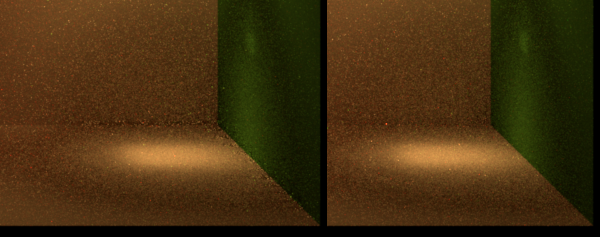
\includegraphics[width=0.8\textwidth]{bilder/kugelbox/caches/artefacts.png}
\caption{Left: camera caches only (3768).\newline
Right: 20k caches including camera caches.\newline
Note how the artefacts vanish on the left where the caustic ends.}
  \label{artefacts}\end{figure}

We also noticed that reducing the number of photon paths resulted in a general noise not unlike the noise from NEE $+$ BSDF sampling, while reducing the number of photons per cache generated a brighter, more colorful noise. Figure \ref{noises} illustrates two extremes that can be gradually improved by increasing the number of photon paths or photons per cache.


 \begin{figure}[h!]
 \centering
 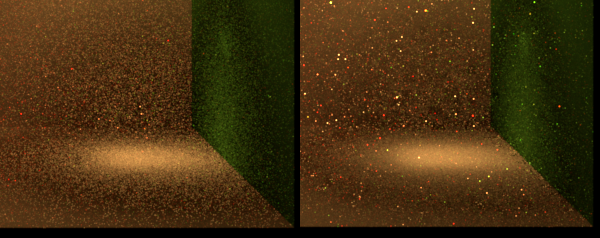
\includegraphics[width=0.8\textwidth]{bilder/kugelbox/caches/different_noises.png}
\caption{Left: 2k photon paths, 3768 caches, 2k photons per cache.\newline
Right: 200k photon paths, 3768 caches, 20 photons per cache.}
  \label{noises}\end{figure}

We settled on around 200k paths and 20k caches with 2k photons each for most of the images shown in section \ref{dcc}, as bigger numbers were not able to improve the images any further. Smaller numbers either produced noise (with less photon paths or photons per cache \ref{noises}) or caused artefacts along edges (too few caches \ref{artefacts}).\\
As a general rule, the number of photon paths should always be at least two orders of magnitude bigger than the number of photons per cache, if we want each cache to only use photons from its immediate surroundings. Our scenes contained an average of 4-8 photons per path. The more open the scene, the smaller this number gets. All our scenes were missing the wall towards the camera; within a completely closed scene there are most likely significantly more photons stored per path.




\subsection{Durations}
\label{durations}

We used an existing library to handle k-d trees and added a cdf to the caches so we could sample points faster using binary search, but apart from that we did not optimize our code in any way.\\
The images were rendered on an Intel i5-3570 CPU with 8GB RAM. The preprocessing of the caches runs in a single thread on one core. The path tracing is multithreaded over 4 cores. We believe the preprocessing step is well suited for parallelization as well, however the main part of the computation time is consumed by the path tracing step anyway.


We measured times for Mitsuba's default path tracer, our path tracer with NEE $+$ BSDF sampling (which does basically the same things as Mitsuba's version) and our path tracer with NEE $+$ IRC sampling. As BSDF $+$ IRC sampling produced the worst results for all of our test scenes, we don't have a detailed list of times for that approach, but it took roughly as long as NEE $+$ IRC sampling.\\
All times are given in minutes. We used 250k photon paths for 20k IRCs with 2500 photons each. The preprocessing time for the IRCs was 1 min and is included in the quoted times.

\begin{table}[h]
\begin{tabular}{|l|llll|}
\hline
                               & Samples per Pixel     & 256  & 512  & 4096  \\ \hline
\multirow{2}{*}{Glass Spheres} & NEE $+$ BSDF sampling & 1.4  & 2.8  & 22.6  \\
                               & NEE $+$ IRC sampling  & 10.9 & 20.7 & 152.1 \\ \hline
\multirow{3}{*}{Glass Egg}     & Mitsuba's path tracer & 3.5  & 7.4  & 58    \\
                               & NEE $+$ BSDF sampling & 4.4  & 8.5  & 71    \\
                               & NEE $+$ IRC sampling  & 19.0 & 37.0 & 281   \\ \hline
\end{tabular}
\end{table}

Observations:

\begin{itemize}
\item Our path tracer (with NEE and BSDF sampling) is not as optimized as Mitsuba's default version. So we believe there is still room for improving the render times.
\item The extra time for NEE $+$ IRC sampling is mainly the result of querying a k-d tree every time the ray intersects the scene. The smaller part is consumed by sampling a direction from the cache.
\item Picking one of the five closest caches resulted in approximately $50\%$ additional render time but no observable difference in the image. As a consequence we only used the closest cache for the listed measurements. All observed artefact problems can also be solved faster by using more caches.
\item For the Glass Spheres scene, NEE $+$ IRC sampling took about 10 times as long as NEE $+$ BSDF sampling, while it only took 4 times as long for the Glass Egg on Table. We assume that the relative overhead for NEE $+$ IRC sampling decreases further with increasing scene complexity, when more time is required to compute ray intersections with the scene.
\end{itemize}
